\documentclass[10pt,a4paper]{article}

% -----------------------------------------------------------------------------
% MATHS MANTHAN | Class 10 Introduction to Trigonometry Master Handbook
% Academic Year 2026--27 | Publication-quality LaTeX source with Vector TikZ.
% Compliant with latest rationalized CBSE curriculum (Complementary angles deleted).
% Compile with pdfLaTeX twice for full resolution of LastPage cross-references.
% -----------------------------------------------------------------------------

\usepackage[a4paper,top=12mm,bottom=16mm,left=15mm,right=15mm,footskip=8mm]{geometry}
\usepackage[T1]{fontenc}
\usepackage{lmodern}
\usepackage{microtype}
\usepackage{amsmath,amssymb}
\usepackage[table]{xcolor}
\usepackage{array,tabularx,booktabs}
\usepackage{graphicx}
\usepackage{eso-pic}
\usepackage{tikz}
\usetikzlibrary{calc,positioning,arrows.meta,shapes.geometric,patterns}
\usepackage[most]{tcolorbox}
\usepackage{enumitem}
\usepackage{fancyhdr}
\usepackage{lastpage}
\usepackage[hidelinks]{hyperref}
\usepackage{url}

% ============================================================================
% BRAND COLOR PALETTE — MATCHED TO THE MATHS MANTHAN STANDARD
% Primary navy: #001F49 | Brand gold: #D19029
% ============================================================================
\definecolor{primary}{RGB}{0,31,73}
\definecolor{brandnavy}{RGB}{0,31,73}
\definecolor{accent}{RGB}{209,144,41}
\definecolor{brandgold}{RGB}{209,144,41}
\definecolor{secondary}{RGB}{75,85,99}
\definecolor{lightgray}{RGB}{246,248,250}
\definecolor{accentlight}{RGB}{254,250,242}
\definecolor{primarylight}{RGB}{240,244,250}

\colorlet{navy}{primary}
\colorlet{blue}{primary!82!black}
\colorlet{gold}{accent}
\colorlet{goldpale}{accentlight}
\colorlet{bluepale}{primarylight}
\colorlet{ink}{secondary}
\colorlet{muted}{secondary}
\colorlet{linegray}{primary!25}
\colorlet{reddeep}{primary}
\colorlet{redpale}{lightgray}
\colorlet{green}{primary}
\colorlet{greenpale}{primarylight}

% -----------------------------------------------------------------------------
% ROBUST LOGO DISCOVERY (TeXworks / pdfLaTeX)
% -----------------------------------------------------------------------------
\graphicspath{{./}}
\newif\ifMMLogoFound
\MMLogoFoundfalse
\def\MMLogoFile{mathsmanthan_logo.png}
\IfFileExists{mathsmanthan_logo.png}{%
  \MMLogoFoundtrue
}{%
  \IfFileExists{mathsmanthan logo.png}{%
    \def\MMLogoFile{mathsmanthan logo.png}%
    \MMLogoFoundtrue
  }{%
    \PackageWarningNoLine{MathsManthan}{Logo image not found. Put mathsmanthan_logo.png in the same folder as this .tex file}%
  }%
}

% Automatic low-opacity logo watermark on every page
\ifMMLogoFound
  \AddToShipoutPictureBG{%
    \begin{tikzpicture}[remember picture,overlay]
      \node[opacity=0.065] at (current page.center) {%
        \includegraphics[width=0.55\paperwidth,keepaspectratio]{\MMLogoFile}%
      };
    \end{tikzpicture}%
  }%
\fi

\hypersetup{
  pdftitle={Class 10 Introduction to Trigonometry | Maths Manthan Handbook},
  pdfauthor={Maths Manthan Tuition Classes},
  pdfsubject={CBSE Class 10 Mathematics, Academic Year 2026--27},
  pdfkeywords={Trigonometry, Class 10, CBSE, Ratios, Identities, Maths Manthan, Formula Handbook}
}

\setlength{\parindent}{0pt}
\setlength{\parskip}{2.5pt}
\renewcommand{\arraystretch}{1.14}
\setlist[itemize]{leftmargin=5mm,itemsep=1.5pt,topsep=1.5pt,parsep=0pt}
\setlist[enumerate]{leftmargin=6mm,itemsep=1.5pt,topsep=1.5pt,parsep=0pt}
\setlength{\tabcolsep}{4.5pt}
\emergencystretch=2em
\hfuzz=1pt

% ============================================================================
% HEADER / FOOTER
% ============================================================================
\newcommand{\TuitionName}{{\color{primary}MATHS} {\color{accent}MANTHAN}}
\newcommand{\TuitionSub}{{\color{primary}\textbullet\ \ \text{TUITION CLASSES}\ \ \textbullet}}
\newcommand{\ContactInfo}{e-mail: contact@mathsmanthan.co.in \quad$\vert$\quad Helpline: +91-8171546558}
\newcommand{\HandbookFooterTitle}{Class 10 Introduction to Trigonometry Handbook}

\pagestyle{fancy}
\fancyhf{}
\renewcommand{\headrulewidth}{0pt}
\renewcommand{\footrulewidth}{0.6pt}
\renewcommand{\footrule}{\hbox to\headwidth{\color{primary!30}\leaders\hrule height 0.6pt\hfill}}
\fancyfoot[L]{\footnotesize\href{https://mathsmanthan.co.in}{\textcolor{secondary}{\TuitionName\ $\vert$\ \HandbookFooterTitle}}}
\fancyfoot[R]{\footnotesize\textbf{\color{primary}Page \thepage\ of \pageref{LastPage}}\quad\textcolor{accent}{\textbf{Academic Year 2026--27}}}

\fancypagestyle{plain}{%
  \fancyhf{}
  \fancyfoot[L]{\footnotesize\href{https://mathsmanthan.co.in}{\textcolor{secondary}{\TuitionName\ $\vert$\ \HandbookFooterTitle}}}
  \fancyfoot[R]{\footnotesize\textbf{\color{primary}Page \thepage\ of \pageref{LastPage}}\quad\textcolor{accent}{\textbf{Academic Year 2026--27}}}
  \renewcommand{\headrulewidth}{0pt}
  \renewcommand{\footrulewidth}{0.6pt}
  \renewcommand{\footrule}{\hbox to\headwidth{\color{primary!30}\leaders\hrule height 0.6pt\hfill}}
}

% Reusable design components
\newcommand{\BrandMark}{%
  \ifMMLogoFound
    \includegraphics[width=22mm,height=22mm,keepaspectratio]{\MMLogoFile}%
  \else
    
\begin{tikzpicture}[baseline=-0.6ex]
      \fill[navy,rounded corners=2.2pt] (0,0) rectangle (1.45,1.05);
      \draw[gold,line width=1.2pt] (0.15,0.15)--(1.30,0.15);
      \node[text=white,font=\sffamily\bfseries\Large] at (0.725,0.59) {MM};
    \end{tikzpicture}%
  \fi
}

\newcommand{\chapterbanner}[4]{%
  \begin{tcolorbox}[enhanced,colback=bluepale,colframe=bluepale,boxrule=0pt,arc=2mm,
    left=4mm,right=4mm,top=2mm,bottom=2mm]
    {\footnotesize\bfseries\color{gold}CHAPTER #1\hfill\color{blue}#4}\par\vspace{0.6mm}
    {\LARGE\bfseries\color{navy}#2}\par
    {\small\color{muted}#3}
  \end{tcolorbox}\vspace{1mm}
}

\newcommand{\subhead}[1]{%
  \vspace{1mm}{\large\bfseries\color{navy}#1}\par\vspace{0.4mm}
  {\color{gold}\rule{13mm}{1.2pt}}\par\vspace{0.8mm}
}

\newtcolorbox{formulaBox}[1][]{enhanced,breakable,colback=goldpale,colframe=gold!65!black,
  boxrule=0.5pt,arc=1.5mm,left=3mm,right=3mm,top=1.8mm,bottom=1.8mm,
  before skip=2.5pt,after skip=3.5pt,#1}
\newtcolorbox{conceptBox}[1][]{enhanced,breakable,colback=bluepale,colframe=blue!25,
  boxrule=0.4pt,arc=1.5mm,left=3mm,right=3mm,top=1.8mm,bottom=1.8mm,
  before skip=2.5pt,after skip=3.5pt,#1}
\newtcolorbox{warningBox}[1][]{enhanced,breakable,colback=redpale,colframe=reddeep!45,
  boxrule=0.45pt,arc=1.5mm,left=3mm,right=3mm,top=1.8mm,bottom=1.8mm,
  before skip=2.5pt,after skip=3.5pt,#1}
\newtcolorbox{successBox}[1][]{enhanced,breakable,colback=greenpale,colframe=green!35,
  boxrule=0.45pt,arc=1.5mm,left=3mm,right=3mm,top=1.8mm,bottom=1.8mm,
  before skip=2.5pt,after skip=3.5pt,#1}

\newcommand{\CoreTag}{\tcbox[colback=greenpale,colframe=green!40,boxrule=.3pt,arc=1mm,left=1.5mm,right=1.5mm,top=.5mm,bottom=.5mm]{\scriptsize\bfseries\color{green}CORE SYLLABUS}}
\newcommand{\ExamTag}{\tcbox[colback=bluepale,colframe=blue!25,boxrule=.3pt,arc=1mm,left=1.5mm,right=1.5mm,top=.5mm,bottom=.5mm]{\scriptsize\bfseries\color{blue}EXAM STRATEGY}}
\newcommand{\TrapTag}{\tcbox[colback=redpale,colframe=reddeep!40,boxrule=.3pt,arc=1mm,left=1.5mm,right=1.5mm,top=.5mm,bottom=.5mm]{\scriptsize\bfseries\color{reddeep}TRAP ALERT}}
\newcommand{\WorkedTag}{\tcbox[colback=bluepale,colframe=blue!25,boxrule=.3pt,arc=1mm,left=1.5mm,right=1.5mm,top=.5mm,bottom=.5mm]{\scriptsize\bfseries\color{blue}WORKED MODEL}}
\newcommand{\SupportTag}{\tcbox[colback=accentlight,colframe=gold!55!black,boxrule=.3pt,arc=1mm,left=1.5mm,right=1.5mm,top=.5mm,bottom=.5mm]{\scriptsize\bfseries\color{primary}SUPPORTING SKILL}}
\newcommand{\ReferenceTag}{\tcbox[colback=bluepale,colframe=blue!25,boxrule=.3pt,arc=1mm,left=1.5mm,right=1.5mm,top=.5mm,bottom=.5mm]{\scriptsize\bfseries\color{primary}REFERENCE MATRIX}}

\begin{document}

% =============================================================================
% PAGE 1: COVER PAGE
% =============================================================================
\thispagestyle{fancy}
\vspace*{0mm}

\noindent
\makebox[0pt][l]{%
  \raisebox{-0.80cm}[0pt][0pt]{%
    \href{https://mathsmanthan.co.in}{%
      \BrandMark%
    }%
  }%
}%
\parbox{\textwidth}{%
  \centering
  \href{https://mathsmanthan.co.in}{%
    {\fontsize{23pt}{23pt}\selectfont\bfseries \TuitionName}\\[3pt]
    {\footnotesize\bfseries \TuitionSub}%
  }\\[2pt]
  {\scriptsize\color{secondary} \ContactInfo}
}

\vspace{5pt}
\noindent{\color{primary}\rule{0.72\textwidth}{1.5pt}}\hfill{\color{accent}\rule{0.26\textwidth}{1.5pt}}

\vspace{3mm}
\begin{center}
  {\large\bfseries\color{muted}CBSE CLASS 10 \;|\; MATHEMATICS}\\[3mm]
  {\fontsize{25}{29}\selectfont\bfseries\color{navy}INTRODUCTION TO TRIGONOMETRY}\\[2mm]
  {\Large\color{blue}Ratios, Exact Values, Transformations \& Pythagorean Identities}\\[2.5mm]
  {\large\color{gold}\bfseries Academic Year 2026--27}
\end{center}

\vspace{2mm}
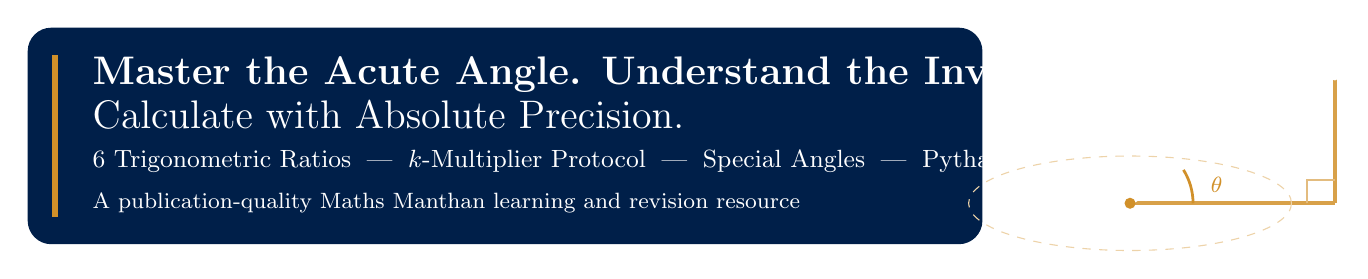
\begin{tikzpicture}
  \fill[navy,rounded corners=3mm] (0,0) rectangle (\textwidth,2.75);
  \draw[gold,line width=2pt] (0.35,0.35)--(0.35,2.40);
  \node[anchor=west,text=white,font=\bfseries\Large] at (0.7,2.15) {Master the Acute Angle. Understand the Invariance.};
  \node[anchor=west,text=white,font=\Large] at (0.7,1.65) {Calculate with Absolute Precision.};
  \node[anchor=west,text=white,font=\small] at (0.7,1.05) {6 Trigonometric Ratios \;|\; $k$-Multiplier Protocol \;|\; Special Angles \;|\; Pythagorean Identities};
  \node[anchor=west,text=white!75,font=\footnotesize] at (0.7,0.52) {A publication-quality Maths Manthan learning and revision resource};
  
  % Decorative Trigonometric Unit Geometry Motif in gold & white
  \draw[gold!85, line width=1.5pt] (14.0, 0.52) -- (16.6, 0.52);
  \draw[gold!85, line width=1.5pt] (16.6, 0.52) -- (16.6, 2.15);
  \draw[white, line width=1.5pt] (14.0, 0.52) -- (16.6, 2.15);
  \draw[gold, line width=1pt] (14.8, 0.52) arc (0:32:0.8);
  \node[text=gold, font=\bfseries\footnotesize] at (15.1, 0.75) {$\theta$};
  \fill[gold] (14.0, 0.52) circle (2pt);
  \fill[white] (16.6, 2.15) circle (2pt);
  \draw[gold!60, line width=0.8pt] (16.25, 0.52) -- (16.25, 0.82) -- (16.6, 0.82);
  \draw[gold!40, dashed] (14.0, 0.52) circle (2.05cm and 0.6cm);
\end{tikzpicture}

\vspace{2.5mm}
\begin{minipage}[t]{0.485\textwidth}
  \begin{conceptBox}[title=What this handbook includes,fonttitle=\bfseries\color{navy}]
    \begin{itemize}
      \item Complete geometric foundations: Opposite (Perpendicular), Adjacent (Base), Hypotenuse, and Orientation Shift.
      \item Scale Invariance Theorem: Why trigonometric ratios depend solely on angle $\theta$ (Thales/AA similarity proof).
      \item The $k$-multiplier evaluation method for finding all ratios from one.
      \item Geometric derivations of $30^\circ, 45^\circ, 60^\circ$ and boundaries $0^\circ, 90^\circ$.
      \item Complete Pythagorean identity derivations and master proving toolkits.
    \end{itemize}
  \end{conceptBox}
\end{minipage}\hfill
\begin{minipage}[t]{0.485\textwidth}
  \begin{formulaBox}[title=How to use it for maximum marks,fonttitle=\bfseries\color{navy}]
    \raggedright Always sketch a neat right-angled triangle and locate the acute reference angle first. When given a numerical ratio (e.g. $\sin A = 3/5$), declare the side lengths with a positive proportionality multiplier $k$ ($3k, 5k$) to protect your method marks. In identity proofs, quote the standard Pythagorean formulas in parentheses alongside each transformation step.
  \end{formulaBox}
\end{minipage}

\vspace{1.5mm}
\begin{warningBox}[title=Official syllabus scope (CBSE Class X 2026--27),fonttitle=\bfseries\color{navy}]
  The published CBSE Class X curriculum for 2026--27 prescribes \textbf{Trigonometric ratios of an acute angle of a right-angled triangle. Proof of their existence (well defined); values of the trigonometric ratios of $30^\circ, 45^\circ, 60^\circ$. Relationships between the ratios. Proof and applications of the identity $\sin^2 A + \cos^2 A = 1$. Only simple identities to be given.} \\
  \textbf{Strictly Excluded Topics (Deleted from Rationalized Syllabus):} \\
  Section 8.4: Trigonometric Ratios of Complementary Angles ($\sin(90^\circ-A)=\cos A$, $\tan(90^\circ-A)=\cot A$, etc.) and Exercise 8.3 of older textbooks are \textbf{completely deleted}. Questions directly requiring complementary angle identities are excluded from the board examination.\par
  {\scriptsize Source: \href{https://cbseacademic.nic.in/web_material/CurriculumMain27/SecPart1/Maths_SecP1X_2026-27.pdf}{CBSE Mathematics Class X Curriculum (2026--27), Unit V: Trigonometry, Chapter 8}.}
\end{warningBox}

\vfill
\begin{center}
  {\small\bfseries\color{navy}Maths Manthan Tuition Classes}\\
  {\footnotesize\color{muted}contact@mathsmanthan.co.in \quad\textbar\quad +91-8171546558}\\
  {\footnotesize\url{https://mathsmanthan.co.in}}\\[2mm]
  {\scriptsize\color{muted}Prepared for learning and revision \;--\; not an official CBSE publication.}
\end{center}

\newpage

% =============================================================================
% PAGE 2: GEOMETRIC FOUNDATIONS & SCALE INVARIANCE
% =============================================================================
\thispagestyle{fancy}
\vspace*{0mm}

\chapterbanner{8}{GEOMETRIC FOUNDATIONS}{Right Triangle Anatomy, Reference Angle Shift \& Scale Invariance}{\CoreTag}

\subhead{Module 1 $\vert$ Anatomy of a Right Triangle \& The Reference Angle Shift}

Trigonometry begins with the right-angled triangle, where side names are strictly relative to the acute angle under consideration:

\begin{itemize}
  \item \textbf{Hypotenuse ($h$):} The side opposite to the right angle ($90^\circ$). It is strictly the longest side of the triangle.
  \item \textbf{Opposite Side / Perpendicular ($p$):} The side directly opposite to the selected acute reference angle $\theta$.
  \item \textbf{Adjacent Side / Base ($b$):} The side that forms the acute angle $\theta$ alongside the hypotenuse.
\end{itemize}

\vspace{0.8mm}
\begin{center}
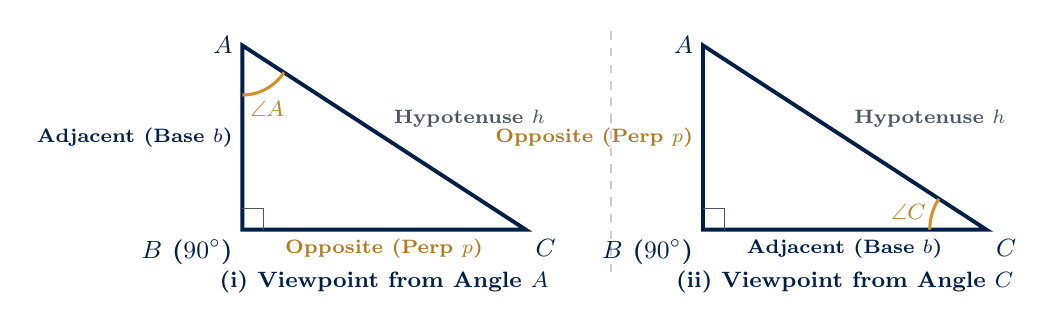
\begin{tikzpicture}[scale=0.9, >=Stealth]
  % Triangle 1: Reference Angle A
  \coordinate (B1) at (0,0);
  \coordinate (A1) at (0,2.6);
  \coordinate (C1) at (4.0,0);
  \draw[navy, line width=1.4pt] (A1) -- (B1) -- (C1) -- cycle;
  \draw[secondary, line width=0.5pt] (0, 0.3) -- (0.3, 0.3) -- (0.3, 0);
  \draw[gold, line width=1.1pt] (0, 1.9) arc (270:327:0.7);
  \node[gold!90!black, font=\bfseries\footnotesize] at (0.35, 1.7) {$\angle A$};
  \node[left, navy, font=\bfseries\small] at (A1) {$A$};
  \node[below left, navy, font=\bfseries\small] at (B1) {$B$ ($90^\circ$)};
  \node[below right, navy, font=\bfseries\small] at (C1) {$C$};
  \node[left, primary, font=\scriptsize\bfseries] at (0, 1.3) {Adjacent (Base $b$)};
  \node[below, gold!85!black, font=\scriptsize\bfseries] at (2.0, 0) {Opposite (Perp $p$)};
  \node[above right, secondary, font=\scriptsize\bfseries] at (2.0, 1.3) {Hypotenuse $h$};
  \node[below, navy, font=\bfseries\footnotesize] at (2.0, -0.45) {\textbf{(i) Viewpoint from Angle $A$}};

  % Divider
  \draw[secondary!30, dashed, line width=0.8pt] (5.2, -0.6) -- (5.2, 2.8);

  % Triangle 2: Reference Angle C
  \coordinate (B2) at (6.5,0);
  \coordinate (A2) at (6.5,2.6);
  \coordinate (C2) at (10.5,0);
  \draw[navy, line width=1.4pt] (A2) -- (B2) -- (C2) -- cycle;
  \draw[secondary, line width=0.5pt] (6.5, 0.3) -- (6.8, 0.3) -- (6.8, 0);
  \draw[gold, line width=1.1pt] (9.7, 0) arc (180:147:0.8);
  \node[gold!90!black, font=\bfseries\footnotesize] at (9.4, 0.25) {$\angle C$};
  \node[left, navy, font=\bfseries\small] at (A2) {$A$};
  \node[below left, navy, font=\bfseries\small] at (B2) {$B$ ($90^\circ$)};
  \node[below right, navy, font=\bfseries\small] at (C2) {$C$};
  \node[left, gold!85!black, font=\scriptsize\bfseries] at (6.5, 1.3) {Opposite (Perp $p$)};
  \node[below, primary, font=\scriptsize\bfseries] at (8.5, 0) {Adjacent (Base $b$)};
  \node[above right, secondary, font=\scriptsize\bfseries] at (8.5, 1.3) {Hypotenuse $h$};
  \node[below, navy, font=\bfseries\footnotesize] at (8.5, -0.45) {\textbf{(ii) Viewpoint from Angle $C$}};
\end{tikzpicture}
\end{center}

\vspace{-1mm}
\subhead{Module 2 $\vert$ The Scale Invariance Theorem: Geometric Well-Definedness}

\begin{conceptBox}[title=Proof of Existence (Well-Definedness of Ratios via AA Similarity),fonttitle=\bfseries\color{navy}]
  \textbf{Fundamental Theorem:} The trigonometric ratios of an acute angle $\theta$ depend \textbf{only} on the measure of angle $\theta$, and are entirely independent of the side lengths or physical dimensions of the triangle. \\
  \textbf{Geometric Proof:} Consider two right-angled triangles $\triangle AB_1 C_1$ and $\triangle AB_2 C_2$ sharing acute angle $\angle A = \theta$:
  $$\angle A = \angle A \quad (\text{Common}), \qquad \angle B_1 = \angle B_2 = 90^\circ$$
  By the AA (Angle-Angle) Similarity Criterion: $\mathbf{\triangle AB_1 C_1 \sim \triangle AB_2 C_2}$. \\
  Therefore, their corresponding sides are strictly proportional:
  $$\mathbf{\frac{B_1 C_1}{B_2 C_2} = \frac{AC_1}{AC_2} = \frac{AB_1}{AB_2} \iff \frac{B_1 C_1}{AC_1} = \frac{B_2 C_2}{AC_2} = \sin\theta}$$
  Thus, whether measured in millimeters or kilometers, the ratio $\frac{\text{Opposite}}{\text{Hypotenuse}}$ is an invariant constant for a given angle $\theta$.
\end{conceptBox}

\vspace{0.5mm}
\begin{center}
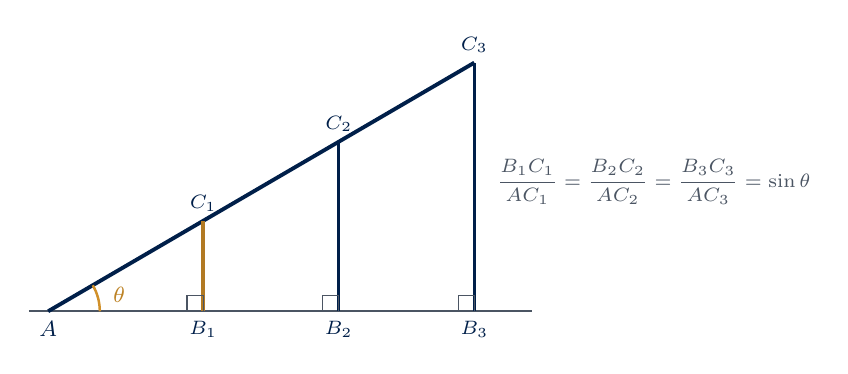
\begin{tikzpicture}[scale=0.82]
  \coordinate (A) at (0,0);
  \coordinate (B1) at (2.4,0);
  \coordinate (C1) at (2.4,1.4);
  \coordinate (B2) at (4.5,0);
  \coordinate (C2) at (4.5,2.625);
  \coordinate (B3) at (6.6,0);
  \coordinate (C3) at (6.6,3.85);

  \draw[thick, secondary] (-0.3,0) -- (7.5,0);
  \draw[navy, line width=1.4pt] (A) -- (C3);
  \draw[gold!85!black, line width=1.2pt] (B1) -- (C1);
  \draw[primary, line width=1.2pt] (B2) -- (C2);
  \draw[navy, line width=1.2pt] (B3) -- (C3);

  \draw[secondary, line width=0.4pt] (2.15,0) rectangle (2.4,0.25);
  \draw[secondary, line width=0.4pt] (4.25,0) rectangle (4.5,0.25);
  \draw[secondary, line width=0.4pt] (6.35,0) rectangle (6.6,0.25);

  \draw[gold, line width=0.9pt] (0.8,0) arc (0:30.2:0.8);
  \node[gold!90!black, font=\bfseries\footnotesize] at (1.1,0.25) {$\theta$};

  \node[below, navy, font=\bfseries\footnotesize] at (A) {$A$};
  \node[below, navy, font=\scriptsize] at (B1) {$B_1$};
  \node[above, navy, font=\scriptsize] at (C1) {$C_1$};
  \node[below, navy, font=\scriptsize] at (B2) {$B_2$};
  \node[above, navy, font=\scriptsize] at (C2) {$C_2$};
  \node[below, navy, font=\scriptsize] at (B3) {$B_3$};
  \node[above, navy, font=\scriptsize] at (C3) {$C_3$};
  \node[right, secondary, font=\scriptsize\itshape] at (6.8, 2.0) {$\dfrac{B_1 C_1}{AC_1} = \dfrac{B_2 C_2}{AC_2} = \dfrac{B_3 C_3}{AC_3} = \sin\theta$};
\end{tikzpicture}
\end{center}

\newpage

% =============================================================================
% PAGE 3: THE SIX TRIGONOMETRIC RATIOS & INTER-RELATIONS
% =============================================================================
\thispagestyle{fancy}
\vspace*{0mm}

\chapterbanner{8}{THE SIX TRIGONOMETRIC RATIOS}{Definitions, Reciprocal Pairs \& Quotient Relations}{\CoreTag}

\subhead{Module 1 $\vert$ Formal Geometric Definitions}

For an acute angle $\theta$ in a right-angled triangle with Opposite ($p$), Adjacent ($b$), and Hypotenuse ($h$):

\begin{center}
{\footnotesize
\begin{tabularx}{\textwidth}{@{}lllX@{}}
  \toprule
  \textbf{\color{navy}Ratio} & \textbf{\color{navy}Symbol} & \textbf{\color{navy}Geometric Ratio} & \textbf{\color{navy}Intuition \& Physical Meaning} \\
  \midrule
  \textbf{Sine} & $\sin \theta$ & $\dfrac{\text{Opposite}}{\text{Hypotenuse}} = \dfrac{p}{h}$ & Fractional vertical elevation achieved per unit hypotenuse. \\
  \addlinespace[1pt]
  \textbf{Cosine} & $\cos \theta$ & $\dfrac{\text{Adjacent}}{\text{Hypotenuse}} = \dfrac{b}{h}$ & Fractional horizontal base covered per unit hypotenuse. \\
  \addlinespace[1pt]
  \textbf{Tangent} & $\tan \theta$ & $\dfrac{\text{Opposite}}{\text{Adjacent}} = \dfrac{p}{b}$ & Geometric steepness or slope (rise over run) of the incline. \\
  \addlinespace[1pt]
  \textbf{Cosecant} & $\csc \theta$ & $\dfrac{\text{Hypotenuse}}{\text{Opposite}} = \dfrac{h}{p}$ & Reciprocal of sine: total travel needed per unit vertical gain. \\
  \addlinespace[1pt]
  \textbf{Secant} & $\sec \theta$ & $\dfrac{\text{Hypotenuse}}{\text{Adjacent}} = \dfrac{h}{b}$ & Reciprocal of cosine: total travel needed per unit horizontal span. \\
  \addlinespace[1pt]
  \textbf{Cotangent} & $\cot \theta$ & $\dfrac{\text{Adjacent}}{\text{Opposite}} = \dfrac{b}{p}$ & Reciprocal of tangent: horizontal run per unit vertical height. \\
  \bottomrule
\end{tabularx}}
\end{center}

\vspace{-1mm}
\subhead{Module 2 $\vert$ Reciprocal Pairs \& Quotient Relations}
\vspace{-1mm}

\begin{formulaBox}[title=Governing Algebraic Inter-Relations,fonttitle=\bfseries\color{navy}]
  \textbf{Reciprocal Identities (Product Equals 1):} \\[1pt]
  $\mathbf{\sin \theta = \frac{1}{\csc \theta} \iff \sin \theta \cdot \csc \theta = 1} \quad\vert\quad \mathbf{\cos \theta = \frac{1}{\sec \theta} \iff \cos \theta \cdot \sec \theta = 1} \quad\vert\quad \mathbf{\tan \theta = \frac{1}{\cot \theta} \iff \tan \theta \cdot \cot \theta = 1}$ \\[3pt]
  \textbf{Quotient Identities (Ratios of Primary Functions):} \\[1pt]
  $\mathbf{\tan \theta = \frac{\sin \theta}{\cos \theta} = \frac{p/h}{b/h} = \frac{p}{b}} \qquad\qquad\qquad\qquad\qquad \mathbf{\cot \theta = \frac{\cos \theta}{\sin \theta} = \frac{b/h}{p/h} = \frac{b}{p}}$
\end{formulaBox}

\vspace{-0.5mm}
\begin{minipage}[t]{0.56\textwidth}
  \subhead{Module 3 $\vert$ Acute Bounds ($0^\circ < \theta < 90^\circ$)}
  \begin{warningBox}[title=Strict Mathematical Bounds,fonttitle=\bfseries\color{navy}]
    Hypotenuse is always strictly the longest side ($h > p$ and $h > b$). Consequently for all acute $\theta$:
    \begin{itemize}[leftmargin=*,itemsep=1pt,topsep=1pt]
      \item $\mathbf{0 < \sin \theta < 1}$ \ and \ $\mathbf{0 < \cos \theta < 1}$ (\textbf{Never} $> 1$).
      \item $\mathbf{\sec \theta > 1}$ \ and \ $\mathbf{\csc \theta > 1}$ (\textbf{Never} $< 1$).
      \item $\mathbf{0 < \tan \theta < \infty}$ \ and \ $\mathbf{0 < \cot \theta < \infty}$.
    \end{itemize}
    \textbf{Trap Alert:} $\sin\theta$ and $\cos\theta$ can \textbf{never} exceed 1!
  \end{warningBox}
\end{minipage}\hfill
\begin{minipage}[t]{0.42\textwidth}
  \begin{center}
  \vspace{2mm}
  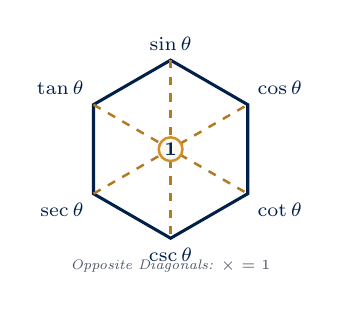
\begin{tikzpicture}[scale=0.78]
    % Hexagon vertices
    \coordinate (S) at (90:1.45);   % sin
    \coordinate (C) at (30:1.45);   % cos
    \coordinate (COT) at (330:1.45);% cot
    \coordinate (CSC) at (270:1.45);% csc
    \coordinate (SEC) at (210:1.45);% sec
    \coordinate (T) at (150:1.45);  % tan

    % Hexagon lines
    \draw[navy, line width=1.1pt] (S) -- (C) -- (COT) -- (CSC) -- (SEC) -- (T) -- cycle;
    % Diagonals
    \draw[gold!85!black, dashed, line width=0.9pt] (S) -- (CSC);
    \draw[gold!85!black, dashed, line width=0.9pt] (T) -- (COT);
    \draw[gold!85!black, dashed, line width=0.9pt] (SEC) -- (C);

    % Central "1" node
    \fill[goldpale] (0,0) circle (5.5pt);
    \draw[gold, line width=0.9pt] (0,0) circle (5.5pt);
    \node[navy, font=\bfseries\scriptsize] at (0,0) {1};

    % Node labels
    \node[above, navy, font=\bfseries\scriptsize] at (S) {$\sin\theta$};
    \node[above right, navy, font=\bfseries\scriptsize] at (C) {$\cos\theta$};
    \node[below right, navy, font=\bfseries\scriptsize] at (COT) {$\cot\theta$};
    \node[below, navy, font=\bfseries\scriptsize] at (CSC) {$\csc\theta$};
    \node[below left, navy, font=\bfseries\scriptsize] at (SEC) {$\sec\theta$};
    \node[above left, navy, font=\bfseries\scriptsize] at (T) {$\tan\theta$};

    \node[below, secondary, font=\tiny\itshape] at (0, -1.65) {Opposite Diagonals: $\times = 1$};
  \end{tikzpicture}
  \end{center}
\end{minipage}

\newpage

% =============================================================================
% PAGE 4: GIVEN ONE RATIO, FIND ALL (THE k-FACTOR PROTOCOL)
% =============================================================================
\thispagestyle{fancy}
\vspace*{0mm}

\chapterbanner{8}{RATIO COMPUTATION PROTOCOLS}{Given One Ratio, Finding All Others: The $k$-Factor Method}{\WorkedTag}

\subhead{Module 1 $\vert$ The Mandatory $k$-Proportionality Rule for Board Exams}

\begin{conceptBox}[title=Why CBSE Examiners Deduct Marks for Missing '$k$',fonttitle=\bfseries\color{navy}]
  \textbf{Critical Concept:} A trigonometric ratio represents the \textbf{relative scale} between two sides, not their absolute physical lengths. For instance, $\sin A = \frac{3}{5}$ means the ratio is $3:5$; sides could be $3\,\text{cm}, 5\,\text{cm}$ or $6\,\text{cm}, 10\,\text{cm}$. \\
  \textbf{Official Marking Scheme Rule:} Writing $\text{Opposite} = 3$ and $\text{Hypotenuse} = 5$ without defining a positive real scaling multiplier $k > 0$ violates dimensional rigor and risks a \textbf{0.5 to 1 mark penalty}. Always state:
  $$\mathbf{\text{Opposite} = 3k \quad \text{and} \quad \text{Hypotenuse} = 5k, \quad \text{where } k > 0}$$
\end{conceptBox}

\vspace{0.4mm}
\subhead{Module 2 $\vert$ Worked Board Archetype 1: Expression Evaluation with Given Cotangent}

\begin{minipage}[t]{0.56\textwidth}
  \textbf{Problem:} If $\cot \theta = \frac{7}{8}$, evaluate: (i) $\frac{(1 + \sin\theta)(1 - \sin\theta)}{(1 + \cos\theta)(1 - \cos\theta)}$, \ (ii) $\cot^2 \theta$. \\
  \textbf{Solution:}\par
  \textbf{Step 1: Declare side lengths with $k$.} \\
  In right $\triangle ABC$, $\cot\theta = \frac{b}{p} = \frac{7}{8}$. Let $b = 7k, p = 8k$ ($k > 0$). \\
  \textbf{Step 2: Hypotenuse by Pythagoras Theorem.} \\
  $h = \sqrt{(8k)^2 + (7k)^2} = \sqrt{64k^2 + 49k^2} = k\sqrt{113}$. \\
  \textbf{Step 3: Algebraic Identity Simplification.} \\
  $\text{Num} = (1 + \sin\theta)(1 - \sin\theta) = 1 - \sin^2\theta = \cos^2\theta$ \\
  $\text{Den} = (1 + \cos\theta)(1 - \cos\theta) = 1 - \cos^2\theta = \sin^2\theta$ \\
  $\therefore \frac{\cos^2\theta}{\sin^2\theta} = \cot^2\theta = \left(\frac{7}{8}\right)^2 = \mathbf{\frac{49}{64}}$. \ Both (i) and (ii) evaluate to $\mathbf{\frac{49}{64}}$.
\end{minipage}\hfill
\begin{minipage}[t]{0.42\textwidth}
  \begin{center}
  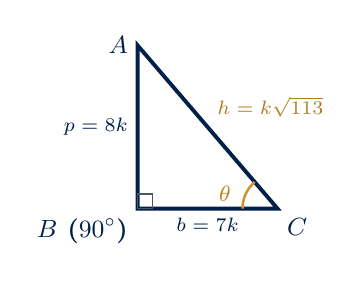
\begin{tikzpicture}[scale=0.74]
    \coordinate (B) at (0,0);
    \coordinate (C) at (2.4,0);
    \coordinate (A) at (0,2.8);

    \draw[navy, line width=1.4pt] (A) -- (B) -- (C) -- cycle;
    \draw[secondary, line width=0.4pt] (0, 0.25) rectangle (0.25, 0);

    \draw[gold, line width=0.9pt] (1.8, 0) arc (180:130.6:0.6);
    \node[gold!90!black, font=\bfseries\footnotesize] at (1.5, 0.25) {$\theta$};

    \node[left, navy, font=\bfseries\small] at (A) {$A$};
    \node[below left, navy, font=\bfseries\small] at (B) {$B$ ($90^\circ$)};
    \node[below right, navy, font=\bfseries\small] at (C) {$C$};

    \node[left, primary, font=\scriptsize\bfseries] at (0, 1.4) {$p = 8k$};
    \node[below, primary, font=\scriptsize\bfseries] at (1.2, 0) {$b = 7k$};
    \node[above right, gold!85!black, font=\scriptsize\bfseries] at (1.2, 1.4) {$h = k\sqrt{113}$};
  \end{tikzpicture}
  \end{center}
\end{minipage}

\vspace{0.4mm}
\subhead{Module 3 $\vert$ Worked Board Archetype 2: Coefficient on Ratio ($15\cot A = 8$)}

\begin{formulaBox}[title=Worked Model: Isolate the Ratio First,fonttitle=\bfseries\color{navy}]
  \textbf{Problem:} Given $15 \cot A = 8$, find the values of $\sin A$ and $\sec A$. \\
  \textbf{Solution:}\par
  \textbf{Step 1: Isolate ratio.} $\cot A = \frac{8}{15} = \frac{\text{Adjacent } b}{\text{Opposite } p}$. Let $b = 8k$ and $p = 15k$ ($k > 0$). \\
  \textbf{Step 2: Hypotenuse.} $h = \sqrt{(15k)^2 + (8k)^2} = \sqrt{225k^2 + 64k^2} = \sqrt{289k^2} = 17k$. \\
  \textbf{Step 3: State desired ratios.} \\[1pt]
  $\mathbf{\sin A = \frac{\text{Opposite}}{\text{Hypotenuse}} = \frac{15k}{17k} = \frac{15}{17}} \qquad\qquad\qquad\qquad \mathbf{\sec A = \frac{\text{Hypotenuse}}{\text{Adjacent}} = \frac{17k}{8k} = \frac{17}{8}}$
\end{formulaBox}

\newpage

% =============================================================================
% PAGE 5: GEOMETRIC DERIVATIONS OF STANDARD ANGLES
% =============================================================================
\thispagestyle{fancy}
\vspace*{0mm}

\chapterbanner{8}{STANDARD ANGLE GEOMETRY}{Geometric Derivations of 45$^\circ$, 30$^\circ$, and 60$^\circ$ Ratios}{\CoreTag}

\subhead{Module 1 $\vert$ Geometric Derivation of Ratios of $45^\circ$ via Isosceles Right Triangle}

\begin{minipage}[t]{0.52\textwidth}
  \textbf{Construction:} Consider an isosceles right $\triangle ABC$ right-angled at $B$ with $\angle A = 45^\circ$.
  \begin{itemize}
    \item By Angle Sum Property: $\angle C = 180^\circ - (90^\circ + 45^\circ) = 45^\circ$.
    \item Equal angles subtend equal sides: $AB = BC = a$.
    \item By Pythagoras Theorem:
      $$AC = \sqrt{AB^2 + BC^2} = \sqrt{a^2 + a^2} = \sqrt{2a^2} = a\sqrt{2}$$
  \end{itemize}
  $$\mathbf{\sin 45^\circ = \frac{1}{\sqrt{2}}}, \qquad \mathbf{\cos 45^\circ = \frac{1}{\sqrt{2}}}, \qquad \mathbf{\tan 45^\circ = 1}$$
  \centerline{\footnotesize\color{secondary}(Reciprocals: $\csc 45^\circ = \sqrt{2}$, \ $\sec 45^\circ = \sqrt{2}$, \ $\cot 45^\circ = 1$)}
\end{minipage}\hfill
\begin{minipage}[t]{0.45\textwidth}
  \begin{center}
  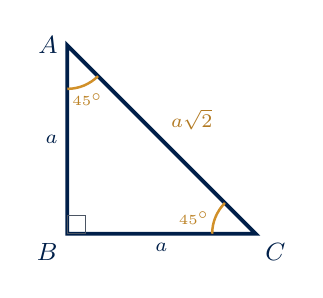
\begin{tikzpicture}[scale=0.92]
    \coordinate (B) at (0,0);
    \coordinate (C) at (2.6,0);
    \coordinate (A) at (0,2.6);

    \draw[navy, line width=1.4pt] (A) -- (B) -- (C) -- cycle;
    \draw[secondary, line width=0.4pt] (0, 0.25) rectangle (0.25, 0);

    \draw[gold, line width=0.9pt] (0, 2.0) arc (270:315:0.6);
    \node[gold!90!black, font=\bfseries\tiny] at (0.28, 1.85) {$45^\circ$};

    \draw[gold, line width=0.9pt] (2.0, 0) arc (180:135:0.6);
    \node[gold!90!black, font=\bfseries\tiny] at (1.75, 0.22) {$45^\circ$};

    \node[left, navy, font=\bfseries\small] at (A) {$A$};
    \node[below left, navy, font=\bfseries\small] at (B) {$B$};
    \node[below right, navy, font=\bfseries\small] at (C) {$C$};

    \node[left, primary, font=\scriptsize\bfseries] at (0, 1.3) {$a$};
    \node[below, primary, font=\scriptsize\bfseries] at (1.3, 0) {$a$};
    \node[above right, gold!85!black, font=\scriptsize\bfseries] at (1.3, 1.3) {$a\sqrt{2}$};
  \end{tikzpicture}
  \end{center}
\end{minipage}

\vspace{0.8mm}
\subhead{Module 2 $\vert$ Geometric Derivation of Ratios of $30^\circ$ and $60^\circ$ via Equilateral Triangle}

\begin{minipage}[t]{0.52\textwidth}
  \textbf{Construction:} Let $\triangle ABD$ be an equilateral triangle with side $2a$. Each angle $= 60^\circ$. Draw altitude $AC \perp BD$.
  \begin{itemize}
    \item Altitude bisects base: $BC = CD = a$.
    \item Altitude bisects vertical angle: $\angle BAC = 30^\circ$.
    \item In right $\triangle ABC$, by Pythagoras Theorem:
      $$AC = \sqrt{(2a)^2 - a^2} = \sqrt{4a^2 - a^2} = \sqrt{3a^2} = a\sqrt{3}$$
  \end{itemize}
  \textbf{Ratios for $30^\circ$ ($p = a$, $b = a\sqrt{3}$, $h = 2a$):}
  $$\mathbf{\sin 30^\circ = \frac{1}{2}}, \qquad \mathbf{\cos 30^\circ = \frac{\sqrt{3}}{2}}, \qquad \mathbf{\tan 30^\circ = \frac{1}{\sqrt{3}}}$$
  \textbf{Ratios for $60^\circ$ ($p = a\sqrt{3}$, $b = a$, $h = 2a$):}
  $$\mathbf{\sin 60^\circ = \frac{\sqrt{3}}{2}}, \qquad \mathbf{\cos 60^\circ = \frac{1}{2}}, \qquad \mathbf{\tan 60^\circ = \sqrt{3}}$$
\end{minipage}\hfill
\begin{minipage}[t]{0.45\textwidth}
  \begin{center}
  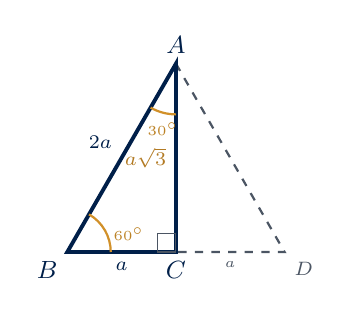
\begin{tikzpicture}[scale=0.92]
    \coordinate (C) at (0,0);
    \coordinate (B) at (-1.5,0);
    \coordinate (D) at (1.5,0);
    \coordinate (A) at (0,2.6);

    \draw[secondary, dashed, line width=0.8pt] (A) -- (D) -- (B);
    \draw[navy, line width=1.4pt] (A) -- (B) -- (C) -- cycle;
    \draw[primary, line width=1.2pt] (A) -- (C);

    \draw[secondary, line width=0.4pt] (-0.25, 0) rectangle (0, 0.25);

    \draw[gold, line width=0.8pt] (-0.9, 0) arc (0:60:0.6);
    \node[gold!90!black, font=\bfseries\tiny] at (-0.65, 0.25) {$60^\circ$};

    \draw[gold, line width=0.8pt] (0, 1.9) arc (270:240:0.7);
    \node[gold!90!black, font=\bfseries\tiny] at (-0.18, 1.7) {$30^\circ$};

    \node[above, navy, font=\bfseries\small] at (A) {$A$};
    \node[below left, navy, font=\bfseries\small] at (B) {$B$};
    \node[below, navy, font=\bfseries\small] at (C) {$C$};
    \node[below right, secondary, font=\scriptsize] at (D) {$D$};

    \node[below, primary, font=\scriptsize\bfseries] at (-0.75, 0) {$a$};
    \node[below, secondary, font=\tiny] at (0.75, 0) {$a$};
    \node[left, gold!85!black, font=\scriptsize\bfseries] at (0, 1.3) {$a\sqrt{3}$};
    \node[above left, navy, font=\scriptsize\bfseries] at (-0.75, 1.3) {$2a$};
  \end{tikzpicture}
  \end{center}
\end{minipage}

\newpage

% =============================================================================
% PAGE 6: MASTER TRIGONOMETRIC VALUES TABLE & SCALING ENGINE
% =============================================================================
\thispagestyle{fancy}
\vspace*{0mm}

\chapterbanner{8}{EXACT VALUES ENGINE}{The Master Angle Table, Monotonicity \& Mental Shortcuts}{\CoreTag}

\subhead{Module 1 $\vert$ The Master Trigonometric Table for Standard Angles}

\begin{center}
{\small
\begin{tabularx}{\textwidth}{@{}lccccc@{}}
  \toprule
  \textbf{\color{navy}Ratio / Angle} & $\mathbf{0^\circ}$ & $\mathbf{30^\circ}$ & $\mathbf{45^\circ}$ & $\mathbf{60^\circ}$ & $\mathbf{90^\circ}$ \\
  \midrule
  $\mathbf{\sin \theta}$ & $\mathbf{0}$ & $\mathbf{\dfrac{1}{2}}$ & $\mathbf{\dfrac{1}{\sqrt{2}} = \dfrac{\sqrt{2}}{2}}$ & $\mathbf{\dfrac{\sqrt{3}}{2}}$ & $\mathbf{1}$ \\
  \addlinespace[2pt]
  $\mathbf{\cos \theta}$ & $\mathbf{1}$ & $\mathbf{\dfrac{\sqrt{3}}{2}}$ & $\mathbf{\dfrac{1}{\sqrt{2}} = \dfrac{\sqrt{2}}{2}}$ & $\mathbf{\dfrac{1}{2}}$ & $\mathbf{0}$ \\
  \addlinespace[2pt]
  $\mathbf{\tan \theta}$ & $\mathbf{0}$ & $\mathbf{\dfrac{1}{\sqrt{3}} = \dfrac{\sqrt{3}}{3}}$ & $\mathbf{1}$ & $\mathbf{\sqrt{3}}$ & \textbf{Not Defined} ($\infty$) \\
  \addlinespace[2pt]
  $\mathbf{\csc \theta}$ & \textbf{Not Defined} & $\mathbf{2}$ & $\mathbf{\sqrt{2}}$ & $\mathbf{\dfrac{2}{\sqrt{3}} = \dfrac{2\sqrt{3}}{3}}$ & $\mathbf{1}$ \\
  \addlinespace[2pt]
  $\mathbf{\sec \theta}$ & $\mathbf{1}$ & $\mathbf{\dfrac{2}{\sqrt{3}} = \dfrac{2\sqrt{3}}{3}}$ & $\mathbf{\sqrt{2}}$ & $\mathbf{2}$ & \textbf{Not Defined} ($\infty$) \\
  \addlinespace[2pt]
  $\mathbf{\cot \theta}$ & \textbf{Not Defined} & $\mathbf{\sqrt{3}}$ & $\mathbf{1}$ & $\mathbf{\dfrac{1}{\sqrt{3}} = \dfrac{\sqrt{3}}{3}}$ & $\mathbf{0}$ \\
  \bottomrule
\end{tabularx}}
\end{center}

\vspace{0.8mm}
\subhead{Module 2 $\vert$ The ``Square Root of Quarters'' Mental Memory Trick}

\begin{formulaBox}[title=5-Second Table Reconstruction Protocol,fonttitle=\bfseries\color{navy}]
  Write the whole numbers $0, 1, 2, 3, 4$ under angles $0^\circ, 30^\circ, 45^\circ, 60^\circ, 90^\circ$, divide each by $4$, and take the square root:
  $$\sin 0^\circ = \sqrt{\frac{0}{4}} = \mathbf{0}, \quad \sin 30^\circ = \sqrt{\frac{1}{4}} = \mathbf{\frac{1}{2}}, \quad \sin 45^\circ = \sqrt{\frac{2}{4}} = \mathbf{\frac{1}{\sqrt{2}}}, \quad \sin 60^\circ = \sqrt{\frac{3}{4}} = \mathbf{\frac{\sqrt{3}}{2}}, \quad \sin 90^\circ = \sqrt{\frac{4}{4}} = \mathbf{1}$$
  To find $\cos\theta$, simply reverse the row order: $1, \frac{\sqrt{3}}{2}, \frac{1}{\sqrt{2}}, \frac{1}{2}, 0$. Then $\tan\theta = \frac{\sin\theta}{\cos\theta}$.
\end{formulaBox}

\vspace{0.5mm}
\begin{minipage}[t]{0.52\textwidth}
  \subhead{Module 3 $\vert$ Monotonicity Trajectories ($0^\circ \le \theta \le 90^\circ$)}
  \begin{conceptBox}[title=Behavior as Angle $\theta$ Increases,fonttitle=\bfseries\color{navy}]
    \begin{itemize}
      \item $\sin\theta$ \textbf{strictly increases} from $0$ to $1$.
      \item $\cos\theta$ \textbf{strictly decreases} from $1$ to $0$.
      \item $\tan\theta$ \textbf{strictly increases} from $0$ to $\infty$.
      \item At $\mathbf{\theta = 45^\circ}$: $\sin 45^\circ = \cos 45^\circ = 1/\sqrt{2}$.
      \item For $\mathbf{\theta < 45^\circ}$: $\cos\theta > \sin\theta$.
      \item For $\mathbf{\theta > 45^\circ}$: $\sin\theta > \cos\theta$.
    \end{itemize}
  \end{conceptBox}
\end{minipage}\hfill
\begin{minipage}[t]{0.45\textwidth}
  \begin{center}
  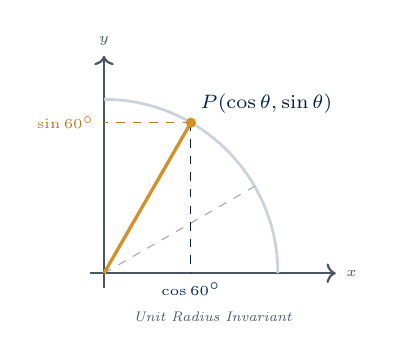
\begin{tikzpicture}[scale=0.92]
    % Coordinate axes
    \draw[thick, secondary, ->] (-0.2,0) -- (3.2,0) node[right, font=\tiny] {$x$};
    \draw[thick, secondary, ->] (0,-0.2) -- (0,3.0) node[above, font=\tiny] {$y$};

    % Quarter circle of radius 2.4
    \draw[primary!20, line width=1pt] (2.4,0) arc (0:90:2.4);

    % Ray at 30 deg
    \draw[secondary!50, dashed] (0,0) -- (30:2.4) coordinate (P30);
    \draw[gold, line width=1.2pt] (0,0) -- (60:2.4) coordinate (P60);

    \draw[primary, dashed] (P60) -- (P60 |- 0,0) coordinate (M60);
    \draw[gold!85!black, dashed] (P60) -- (P60 -| 0,0) coordinate (N60);

    \node[below, navy, font=\tiny] at (M60) {$\cos 60^\circ$};
    \node[left, gold!85!black, font=\tiny] at (N60) {$\sin 60^\circ$};

    \fill[gold] (P60) circle (2pt);
    \node[above right, navy, font=\scriptsize\bfseries] at (P60) {$P(\cos\theta, \sin\theta)$};

    \node[below, secondary, font=\tiny\itshape] at (1.5, -0.4) {Unit Radius Invariant};
  \end{tikzpicture}
  \end{center}
\end{minipage}

\newpage

% =============================================================================
% PAGE 7: NUMERICAL EVALUATION OF TRIGONOMETRIC EXPRESSIONS
% =============================================================================
\thispagestyle{fancy}
\vspace*{0mm}

\chapterbanner{8}{NUMERICAL EVALUATION}{Order of Operations, Quadratic Powers \& Linear Systems}{\WorkedTag}

\subhead{Module 1 $\vert$ Power Notation \& Evaluation Rules}

\begin{formulaBox}[title=Standard Power Notation Protocol,fonttitle=\bfseries\color{navy}]
  $$\mathbf{\sin^2 \theta \equiv (\sin\theta)^2}, \qquad \mathbf{\cos^n \theta \equiv (\cos\theta)^n}, \qquad \mathbf{\tan^2 \theta \equiv (\tan\theta)^2}$$
  \textbf{Fatal Notation Trap:} $\sin^2\theta$ does \textbf{NOT} mean $\sin(\theta^2)$. For example, $\sin^2 30^\circ = (\sin 30^\circ)^2 = (1/2)^2 = 1/4$, whereas $\sin(30^\circ)^2 = \sin(900^\circ)$ which is an entirely different quantity!
\end{formulaBox}

\vspace{0.4mm}
\subhead{Module 2 $\vert$ Worked Board Archetype 1: Multi-Term Surd Evaluation}

\begin{conceptBox}[title=Worked Model: Comprehensive Fractional Evaluation,fonttitle=\bfseries\color{navy}]
  \textbf{Problem:} Evaluate the exact numerical value of:
  $$E = \frac{5\cos^2 60^\circ + 4\sec^2 30^\circ - \tan^2 45^\circ}{\sin^2 30^\circ + \cos^2 30^\circ}$$
  \textbf{Solution:}\par
  \textbf{Step 1: Substitute exact values into numerator.} \\
  $\cos 60^\circ = \frac{1}{2} \implies \cos^2 60^\circ = \frac{1}{4}; \quad \sec 30^\circ = \frac{2}{\sqrt{3}} \implies \sec^2 30^\circ = \frac{4}{3}; \quad \tan 45^\circ = 1 \implies \tan^2 45^\circ = 1$. \\
  $\text{Numerator} = 5\left(\frac{1}{4}\right) + 4\left(\frac{4}{3}\right) - 1 = \frac{5}{4} + \frac{16}{3} - 1 = \frac{15 + 64 - 12}{12} = \frac{67}{12}$. \\[2pt]
  \textbf{Step 2: Evaluate denominator (Pythagorean identity confirmation).} \\
  $\text{Denominator} = \sin^2 30^\circ + \cos^2 30^\circ = \left(\frac{1}{2}\right)^2 + \left(\frac{\sqrt{3}}{2}\right)^2 = \frac{1}{4} + \frac{3}{4} = 1$. \\[2pt]
  \textbf{Step 3: Compute final quotient.} \\
  $$E = \frac{67/12}{1} = \mathbf{\frac{67}{12}} = \mathbf{5\frac{7}{12}}$$
\end{conceptBox}

\vspace{0.4mm}
\subhead{Module 3 $\vert$ Worked Board Archetype 2: System of Trigonometric Equations}

\begin{conceptBox}[title=Worked Model: Determining Acute Angles $A$ and $B$,fonttitle=\bfseries\color{navy}]
  \textbf{Problem:} If $\tan(A + B) = \sqrt{3}$ and $\tan(A - B) = \frac{1}{\sqrt{3}}$, where $0^\circ < A + B \le 90^\circ$ and $A > B$, find acute angles $A$ and $B$. \\
  \textbf{Solution:}\par
  \textbf{Step 1: Translate trigonometric equations into linear equations.} \\
  $\tan(A + B) = \sqrt{3} = \tan 60^\circ \implies \mathbf{A + B = 60^\circ} \quad \text{--- (1)}$; \qquad $\tan(A - B) = \frac{1}{\sqrt{3}} = \tan 30^\circ \implies \mathbf{A - B = 30^\circ} \quad \text{--- (2)}$. \\[2pt]
  \textbf{Step 2: Solve simultaneously by elimination.} \\
  $\text{Adding (1) and (2): } 2A = 90^\circ \implies \mathbf{A = 45^\circ}$. \qquad $\text{Subtracting (2) from (1): } 2B = 30^\circ \implies \mathbf{B = 15^\circ}$. \\
  \textbf{Final Statement:} $A = \mathbf{45^\circ}$ and $B = \mathbf{15^\circ}$. Both are acute and satisfy $A + B = 60^\circ \le 90^\circ$.
\end{conceptBox}

\newpage

% =============================================================================
% PAGE 8: THE FUNDAMENTAL PYTHAGOREAN IDENTITIES
% =============================================================================
\thispagestyle{fancy}
\vspace*{0mm}

\chapterbanner{8}{PYTHAGOREAN IDENTITIES}{Geometric Derivation, Branching Formulas \& Conjugates}{\CoreTag}

\subhead{Module 1 $\vert$ Mathematical Meaning of an Identity}

An equation is called an \textbf{identity} when it is true for all values of the variables for which the functions are defined.

\subhead{Module 2 $\vert$ Geometric Derivation of the Primary Pythagorean Identity}

\begin{minipage}[t]{0.52\textwidth}
  Consider right $\triangle ABC$ right-angled at $B$ with acute angle $\angle A = \theta$:
  \begin{itemize}
    \item By Pythagoras Theorem:
      $$AB^2 + BC^2 = AC^2$$
    \item Dividing each term by $AC^2$:
      $$\frac{AB^2}{AC^2} + \frac{BC^2}{AC^2} = \frac{AC^2}{AC^2} \implies \left(\frac{AB}{AC}\right)^2 + \left(\frac{BC}{AC}\right)^2 = 1$$
    \item Since $\frac{AB}{AC} = \cos A$ and $\frac{BC}{AC} = \sin A$:
  \end{itemize}
  $$\mathbf{\sin^2 A + \cos^2 A = 1}$$
\end{minipage}\hfill
\begin{minipage}[t]{0.45\textwidth}
  \begin{center}
  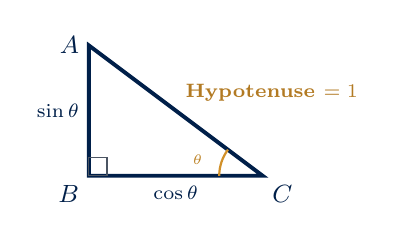
\begin{tikzpicture}[scale=0.92]
    \coordinate (B) at (0,0);
    \coordinate (C) at (2.4,0);
    \coordinate (A) at (0,1.8);

    \draw[navy, line width=1.4pt] (A) -- (B) -- (C) -- cycle;
    \draw[secondary, line width=0.4pt] (0, 0.25) rectangle (0.25, 0);

    \node[left, navy, font=\bfseries\small] at (A) {$A$};
    \node[below left, navy, font=\bfseries\small] at (B) {$B$};
    \node[below right, navy, font=\bfseries\small] at (C) {$C$};

    \draw[gold, line width=0.8pt] (1.8, 0) arc (180:143:0.6);
    \node[gold!90!black, font=\bfseries\tiny] at (1.5, 0.22) {$\theta$};

    \node[left, primary, font=\scriptsize\bfseries] at (0, 0.9) {$\sin\theta$};
    \node[below, primary, font=\scriptsize\bfseries] at (1.2, 0) {$\cos\theta$};
    \node[above right, gold!85!black, font=\scriptsize\bfseries] at (1.2, 0.9) {Hypotenuse $= 1$};
  \end{tikzpicture}
  \end{center}
\end{minipage}

\vspace{0.8mm}
\subhead{Module 3 $\vert$ The Three Sibling Identities \& Difference-of-Squares Branching}

\begin{formulaBox}[title=Master Identity Triad \& Algebraic Conjugate Factors,fonttitle=\bfseries\color{navy}]
  \textbf{1. Sine-Cosine Identity:} Valid for all acute angles $0^\circ \le \theta \le 90^\circ$:
  $$\mathbf{\sin^2\theta + \cos^2\theta = 1} \iff \mathbf{\sin^2\theta = 1 - \cos^2\theta} \iff \mathbf{\cos^2\theta = 1 - \sin^2\theta}$$
  \textbf{2. Tangent-Secant Identity:} Valid for $0^\circ \le \theta < 90^\circ$ (dividing primary identity by $\cos^2\theta$):
  $$\mathbf{1 + \tan^2\theta = \sec^2\theta} \iff \mathbf{\sec^2\theta - \tan^2\theta = 1}$$
  $$\mathbf{(\sec\theta - \tan\theta)(\sec\theta + \tan\theta) = 1 \iff \sec\theta - \tan\theta = \frac{1}{\sec\theta + \tan\theta}}$$
  \textbf{3. Cotangent-Cosecant Identity:} Valid for $0^\circ < \theta \le 90^\circ$ (dividing primary identity by $\sin^2\theta$):
  $$\mathbf{1 + \cot^2\theta = \csc^2\theta} \iff \mathbf{\csc^2\theta - \cot^2\theta = 1}$$
  $$\mathbf{(\csc\theta - \cot\theta)(\csc\theta + \cot\theta) = 1 \iff \csc\theta - \cot\theta = \frac{1}{\csc\theta + \cot\theta}}$$
  \textbf{Golden Exam Hack:} If $\sec\theta + \tan\theta = x$, then instantly $\sec\theta - \tan\theta = \frac{1}{x}$, allowing immediate linear addition to solve for $\sec\theta = \frac{1}{2}(x + \frac{1}{x})$!
\end{formulaBox}

\newpage

% =============================================================================
% PAGE 9: UNIVERSAL RATIO CONVERSION MATRIX
% =============================================================================
\thispagestyle{fancy}
\vspace*{0mm}

\chapterbanner{8}{RATIO CONVERSION MATRIX}{Expressing Any Trigonometric Ratio in Terms of Any Other}{\ReferenceTag}

\subhead{Module 1 $\vert$ The Parameterized Reference Triangle Method}

\begin{minipage}[t]{0.52\textwidth}
  \textbf{Pedagogical Strategy:} The fastest, safest board-exam technique to express all trigonometric ratios in terms of a single target ratio (e.g. $\sec A$) is constructing a \textbf{parameterized right triangle}. \\
  To write all ratios in terms of $\mathbf{\sec A}$:
  \begin{itemize}
    \item Set $\sec A = \frac{\sec A}{1} = \frac{\text{Hypotenuse}}{\text{Adjacent (Base)}}$.
    \item Let $\text{Base} = 1$ and $\text{Hypotenuse} = \sec A$.
    \item By Pythagoras Theorem:
      $$\text{Opposite } p = \sqrt{\sec^2 A - 1}$$
  \end{itemize}
  Every ratio is now read directly from the triangle!
\end{minipage}\hfill
\begin{minipage}[t]{0.45\textwidth}
  \begin{center}
  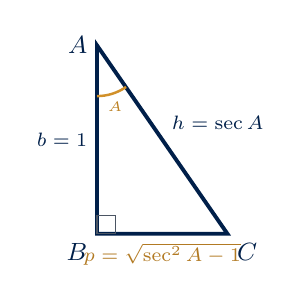
\begin{tikzpicture}[scale=0.92]
    \coordinate (B) at (0,0);
    \coordinate (C) at (1.8,0);
    \coordinate (A) at (0,2.6);

    \draw[navy, line width=1.4pt] (A) -- (B) -- (C) -- cycle;
    \draw[secondary, line width=0.4pt] (0, 0.25) rectangle (0.25, 0);

    \draw[gold, line width=0.9pt] (0, 1.9) arc (270:305:0.7);
    \node[gold!90!black, font=\bfseries\tiny] at (0.25, 1.75) {$A$};

    \node[left, navy, font=\bfseries\small] at (A) {$A$};
    \node[below left, navy, font=\bfseries\small] at (B) {$B$};
    \node[below right, navy, font=\bfseries\small] at (C) {$C$};

    \node[left, primary, font=\scriptsize\bfseries] at (0, 1.3) {$b = 1$};
    \node[below, gold!85!black, font=\scriptsize\bfseries] at (0.9, 0) {$p = \sqrt{\sec^2 A - 1}$};
    \node[above right, navy, font=\scriptsize\bfseries] at (0.9, 1.3) {$h = \sec A$};
  \end{tikzpicture}
  \end{center}
\end{minipage}

\vspace{0.8mm}
\subhead{Module 2 $\vert$ Master 6$\times$6 Universal Ratio Transformation Matrix}

All ratios for an acute angle $A$ expressed in terms of each column's designated generator:

\begin{center}
{\small
\begin{tabularx}{\textwidth}{@{}lcccc@{}}
  \toprule
  \textbf{\color{navy}Ratio} & \textbf{\color{navy}In terms of $\sin A$} & \textbf{\color{navy}In terms of $\cos A$} & \textbf{\color{navy}In terms of $\tan A$} & \textbf{\color{navy}In terms of $\sec A$} \\
  \midrule
  $\mathbf{\sin A}$ & $\sin A$ & $\sqrt{1 - \cos^2 A}$ & $\dfrac{\tan A}{\sqrt{1 + \tan^2 A}}$ & $\dfrac{\sqrt{\sec^2 A - 1}}{\sec A}$ \\
  \addlinespace[2.5pt]
  $\mathbf{\cos A}$ & $\sqrt{1 - \sin^2 A}$ & $\cos A$ & $\dfrac{1}{\sqrt{1 + \tan^2 A}}$ & $\dfrac{1}{\sec A}$ \\
  \addlinespace[2.5pt]
  $\mathbf{\tan A}$ & $\dfrac{\sin A}{\sqrt{1 - \sin^2 A}}$ & $\dfrac{\sqrt{1 - \cos^2 A}}{\cos A}$ & $\tan A$ & $\sqrt{\sec^2 A - 1}$ \\
  \addlinespace[2.5pt]
  $\mathbf{\csc A}$ & $\dfrac{1}{\sin A}$ & $\dfrac{1}{\sqrt{1 - \cos^2 A}}$ & $\dfrac{\sqrt{1 + \tan^2 A}}{\tan A}$ & $\dfrac{\sec A}{\sqrt{\sec^2 A - 1}}$ \\
  \addlinespace[2.5pt]
  $\mathbf{\sec A}$ & $\dfrac{1}{\sqrt{1 - \sin^2 A}}$ & $\dfrac{1}{\cos A}$ & $\sqrt{1 + \tan^2 A}$ & $\sec A$ \\
  \addlinespace[2.5pt]
  $\mathbf{\cot A}$ & $\dfrac{\sqrt{1 - \sin^2 A}}{\sin A}$ & $\dfrac{\cos A}{\sqrt{1 - \cos^2 A}}$ & $\dfrac{1}{\tan A}$ & $\dfrac{1}{\sqrt{\sec^2 A - 1}}$ \\
  \bottomrule
\end{tabularx}}
\end{center}

\vspace{0.8mm}
\begin{conceptBox}[title=Worked Model: Expressing Ratios in terms of $\sec A$ (NCERT Standard),fonttitle=\bfseries\color{navy}]
  \textbf{Task:} Write all other trigonometric ratios of $\angle A$ in terms of $\sec A$. \\
  \textbf{Solution:} Using $\cos A = \frac{1}{\sec A}$, $\sin A = \sqrt{1 - \cos^2 A} = \sqrt{1 - \frac{1}{\sec^2 A}} = \frac{\sqrt{\sec^2 A - 1}}{\sec A}$, $\tan A = \sqrt{\sec^2 A - 1}$, $\cot A = \frac{1}{\tan A} = \frac{1}{\sqrt{\sec^2 A - 1}}$, and $\csc A = \frac{1}{\sin A} = \frac{\sec A}{\sqrt{\sec^2 A - 1}}$.
\end{conceptBox}

\newpage

% =============================================================================
% PAGE 10: IDENTITY PROOF STRATEGIES & WORKED MODELS
% =============================================================================
\thispagestyle{fancy}
\vspace*{0mm}

\chapterbanner{8}{IDENTITY PROOF STRATEGIES}{The 4 Cardinal Techniques \& High-Scoring Board Archetypes}{\WorkedTag}

\subhead{Module 1 $\vert$ The Four Cardinal Proof Strategies}

\begin{formulaBox}[title=The Maths Manthan Universal Identity Solving Protocol,fonttitle=\bfseries\color{navy}]
  \begin{enumerate}
    \item \textbf{Strategy 1 (Sines \& Cosines Default):} Convert compound functions ($\tan, \cot, \sec, \csc$) into pure sines and cosines. This resolves over $70\%$ of board problems into elementary fraction addition.
    \item \textbf{Strategy 2 (Conjugate Rationalization):} When you see denominators like $(1 \pm \sin A)$ or $(1 \pm \cos A)$ or $(\sec A \pm \tan A)$, multiply numerator and denominator by the conjugate to produce a difference of squares!
    \item \textbf{Strategy 3 (Algebraic Factoring):} Look for $a^2 - b^2 = (a-b)(a+b)$ and $a^3 \pm b^3 = (a \pm b)(a^2 \mp ab + b^2)$.
    \item \textbf{Strategy 4 (Dual-Sided Simplification):} When direct LHS $\to$ RHS path is algebraically opaque, reduce LHS to an intermediate simplest form $M$, then reduce RHS independently to the exact same form $M$.
  \end{enumerate}
\end{formulaBox}

\vspace{0.8mm}
\subhead{Module 2 $\vert$ Worked Board Archetype 1: Radical Conjugate Identity}

\begin{conceptBox}[title=Worked Classic Model: Square Root Conjugate Rationalization,fonttitle=\bfseries\color{navy}]
  \textbf{Problem:} Prove that: $\mathbf{\sqrt{\frac{1 + \sin A}{1 - \sin A}} = \sec A + \tan A}$. \\
  \textbf{Proof:}\par
  \textbf{Step 1: Multiply numerator and denominator under radical by conjugate $(1 + \sin A)$.}
  $$\text{LHS} = \sqrt{\frac{1 + \sin A}{1 - \sin A} \times \frac{1 + \sin A}{1 + \sin A}} = \sqrt{\frac{(1 + \sin A)^2}{1 - \sin^2 A}}$$
  \textbf{Step 2: Apply Pythagorean identity $1 - \sin^2 A = \cos^2 A$.}
  $$\text{LHS} = \sqrt{\frac{(1 + \sin A)^2}{\cos^2 A}} = \frac{1 + \sin A}{\cos A}$$
  \textbf{Step 3: Split the fraction into independent terms.}
  $$\text{LHS} = \frac{1}{\cos A} + \frac{\sin A}{\cos A} = \sec A + \tan A = \mathbf{\text{RHS}} \qquad [\textbf{Hence Proved}]$$
\end{conceptBox}

\vspace{0.8mm}
\subhead{Module 3 $\vert$ Worked Board Archetype 2: The $\csc A + \cot A$ Identity Transformation}

\begin{conceptBox}[title=Worked Classic Model: Dividing by Sine \& Factoring Unity,fonttitle=\bfseries\color{navy}]
  \textbf{Problem:} Prove that: $\mathbf{\frac{\cos A - \sin A + 1}{\cos A + \sin A - 1} = \csc A + \cot A}$ using the identity $\csc^2 A = 1 + \cot^2 A$. \\
  \textbf{Proof:}\par
  \textbf{Step 1: Divide every term in numerator and denominator by $\sin A$.}
  $$\text{LHS} = \frac{\frac{\cos A}{\sin A} - \frac{\sin A}{\sin A} + \frac{1}{\sin A}}{\frac{\cos A}{\sin A} + \frac{\sin A}{\sin A} - \frac{1}{\sin A}} = \frac{\cot A - 1 + \csc A}{\cot A + 1 - \csc A} = \frac{(\cot A + \csc A) - 1}{(\cot A - \csc A) + 1}$$
  \textbf{Step 2: Substitute $1 = \csc^2 A - \cot^2 A$ into the numerator.}
  $$\text{LHS} = \frac{(\csc A + \cot A) - (\csc^2 A - \cot^2 A)}{\cot A - \csc A + 1} = \frac{(\csc A + \cot A) - [(\csc A - \cot A)(\csc A + \cot A)]}{\cot A - \csc A + 1}$$
  \textbf{Step 3: Factor out the common binomial $(\csc A + \cot A)$.}
  $$\text{LHS} = \frac{(\csc A + \cot A)[1 - (\csc A - \cot A)]}{1 - \csc A + \cot A} = \frac{(\csc A + \cot A)(1 - \csc A + \cot A)}{1 - \csc A + \cot A} = \mathbf{\csc A + \cot A = \text{RHS}}$$
\end{conceptBox}

\newpage

% =============================================================================
% PAGE 11: ADVANCED BOARD IDENTITY PROVING ARCHETYPES
% =============================================================================
\thispagestyle{fancy}
\vspace*{0mm}

\chapterbanner{8}{ADVANCED IDENTITIES}{Complex Algebraic Manipulations \& 5-Marker Board Models}{\WorkedTag}

\subhead{Module 1 $\vert$ Worked Board Archetype 3: The Tangent-Cotangent Cubic Identity}

\begin{conceptBox}[title=Worked 5-Marker Masterpiece: The Cubic Factorization Route,fonttitle=\bfseries\color{navy}]
  \textbf{Problem:} Prove that: $\mathbf{\frac{\tan\theta}{1 - \cot\theta} + \frac{\cot\theta}{1 - \tan\theta} = 1 + \sec\theta\csc\theta}$. \\
  \textbf{Proof:}\par
  \textbf{Step 1: Convert all functions to pure sines and cosines.}
  $$\text{LHS} = \frac{\frac{\sin\theta}{\cos\theta}}{1 - \frac{\cos\theta}{\sin\theta}} + \frac{\frac{\cos\theta}{\sin\theta}}{1 - \frac{\sin\theta}{\cos\theta}} = \frac{\frac{\sin\theta}{\cos\theta}}{\frac{\sin\theta - \cos\theta}{\sin\theta}} + \frac{\frac{\cos\theta}{\sin\theta}}{\frac{\cos\theta - \sin\theta}{\cos\theta}}$$
  $$\text{LHS} = \frac{\sin^2\theta}{\cos\theta(\sin\theta - \cos\theta)} + \frac{\cos^2\theta}{\sin\theta(\cos\theta - \sin\theta)}$$
  \textbf{Step 2: Align denominators by factoring a minus sign from $(\cos\theta - \sin\theta)$.}
  $$\text{LHS} = \frac{\sin^2\theta}{\cos\theta(\sin\theta - \cos\theta)} - \frac{\cos^2\theta}{\sin\theta(\sin\theta - \cos\theta)}$$
  \textbf{Step 3: Combine over the common denominator $\sin\theta\cos\theta(\sin\theta - \cos\theta)$.}
  $$\text{LHS} = \frac{\sin^3\theta - \cos^3\theta}{\sin\theta\cos\theta(\sin\theta - \cos\theta)}$$
  \textbf{Step 4: Factor numerator using difference of cubes: $a^3 - b^3 = (a - b)(a^2 + ab + b^2)$.}
  $$\text{LHS} = \frac{(\sin\theta - \cos\theta)(\sin^2\theta + \sin\theta\cos\theta + \cos^2\theta)}{\sin\theta\cos\theta(\sin\theta - \cos\theta)}$$
  \textbf{Step 5: Cancel common factor and substitute $\sin^2\theta + \cos^2\theta = 1$.}
  $$\text{LHS} = \frac{1 + \sin\theta\cos\theta}{\sin\theta\cos\theta} = \frac{1}{\sin\theta\cos\theta} + \frac{\sin\theta\cos\theta}{\sin\theta\cos\theta} = \mathbf{1 + \sec\theta\csc\theta = \text{RHS}} \qquad [\textbf{Hence Proved}]$$
\end{conceptBox}

\vspace{0.8mm}
\subhead{Module 2 $\vert$ Worked Board Archetype 4: Expanding Squared Binomials}

\begin{conceptBox}[title=Worked 4-Marker Board Model: Perfect Square Expansion,fonttitle=\bfseries\color{navy}]
  \textbf{Problem:} Prove that: $\mathbf{(\sin A + \csc A)^2 + (\cos A + \sec A)^2 = 7 + \tan^2 A + \cot^2 A}$. \\
  \textbf{Proof:}\par
  \textbf{Step 1: Expand both binomial squares using $(a + b)^2 = a^2 + 2ab + b^2$.}
  $$\text{LHS} = (\sin^2 A + 2\sin A\csc A + \csc^2 A) + (\cos^2 A + 2\cos A\sec A + \sec^2 A)$$
  \textbf{Step 2: Apply reciprocal relations $\sin A\csc A = 1$ and $\cos A\sec A = 1$.}
  $$\text{LHS} = \sin^2 A + 2(1) + \csc^2 A + \cos^2 A + 2(1) + \sec^2 A$$
  \textbf{Step 3: Regroup $(\sin^2 A + \cos^2 A = 1)$ and collect integer constants.}
  $$\text{LHS} = (\sin^2 A + \cos^2 A) + 2 + 2 + \csc^2 A + \sec^2 A = 1 + 4 + \csc^2 A + \sec^2 A = 5 + \csc^2 A + \sec^2 A$$
  \textbf{Step 4: Substitute identities $\csc^2 A = 1 + \cot^2 A$ and $\sec^2 A = 1 + \tan^2 A$.}
  $$\text{LHS} = 5 + (1 + \cot^2 A) + (1 + \tan^2 A) = \mathbf{7 + \tan^2 A + \cot^2 A = \text{RHS}} \qquad [\textbf{Hence Proved}]$$
\end{conceptBox}

\newpage

% =============================================================================
% PAGE 12: MASTER QUICK-REVISION REFERENCE MATRIX
% =============================================================================
\thispagestyle{fancy}
\vspace*{0mm}

\chapterbanner{8}{QUICK-REVISION MATRIX}{Core Laws, Formula Matrix \& Curriculum Clarifications}{\ReferenceTag}

\subhead{Module 1 $\vert$ Comprehensive Trigonometry Formula Reference Matrix}

{\renewcommand{\arraystretch}{1.12}\small
\begin{tabularx}{\textwidth}{@{}lllX@{}}
  \toprule
  \textbf{\color{navy}Category} & \textbf{\color{navy}Primary Relation} & \textbf{\color{navy}Alternative Forms} & \textbf{\color{navy}Exam Application \& Memory Hook} \\
  \midrule
  \textbf{Reciprocals} & $\sin\theta = 1/\csc\theta$ & $\sin\theta \cdot \csc\theta = 1$ & Product of reciprocal pairs always equals $1$. \\
  & $\cos\theta = 1/\sec\theta$ & $\cos\theta \cdot \sec\theta = 1$ & Use when secant/cosecant appears in denominator. \\
  & $\tan\theta = 1/\cot\theta$ & $\tan\theta \cdot \cot\theta = 1$ & Always invert to switch between slope and co-slope. \\
  \addlinespace[1.5pt]
  \textbf{Quotients} & $\tan\theta = \sin\theta/\cos\theta$ & $\cot\theta = \cos\theta/\sin\theta$ & Universal Strategy: Express non-sine/cos in quotients. \\
  \addlinespace[1.5pt]
  \textbf{Identity 1} & $\sin^2\theta + \cos^2\theta = 1$ & $\sin^2\theta = 1 - \cos^2\theta$ & Replaces sum of squares with unity; factor $(1-\cos)(1+\cos)$. \\
  & & $\cos^2\theta = 1 - \sin^2\theta$ & \\
  \addlinespace[1.5pt]
  \textbf{Identity 2} & $1 + \tan^2\theta = \sec^2\theta$ & $\sec^2\theta - \tan^2\theta = 1$ & Conjugate pair: $(\sec\theta - \tan\theta)(\sec\theta + \tan\theta) = 1$. \\
  & & $\tan^2\theta = \sec^2\theta - 1$ & \\
  \addlinespace[1.5pt]
  \textbf{Identity 3} & $1 + \cot^2\theta = \csc^2\theta$ & $\csc^2\theta - \cot^2\theta = 1$ & Conjugate pair: $(\csc\theta - \cot\theta)(\csc\theta + \cot\theta) = 1$. \\
  & & $\cot^2\theta = \csc^2\theta - 1$ & \\
  \addlinespace[1.5pt]
  \textbf{Special Values} & $\sin 30^\circ = \cos 60^\circ = 1/2$ & $\tan 45^\circ = \cot 45^\circ = 1$ & Symmetry points: complementary values are equal. \\
  & $\sin 60^\circ = \cos 30^\circ = \sqrt{3}/2$ & $\sin 45^\circ = \cos 45^\circ = \sqrt{2}/2$ & \\
  \bottomrule
\end{tabularx}}

\vspace{1mm}
\subhead{Module 2 $\vert$ Geometric Symmetry \& Value Invariance}

\begin{conceptBox}[title=Scale Invariance \& Triangle Symmetries,fonttitle=\bfseries\color{navy}]
  \begin{itemize}
    \item \textbf{Similarity Invariance:} If triangle sides are doubled or halved, all 6 trigonometric ratios remain identical.
    \item \textbf{Complementary Acute Angle Symmetry:} In any right triangle $ABC$ with $\angle B = 90^\circ$, acute angles are complementary: $A + C = 90^\circ$. This explains why side $BC$ is Opposite to $A$ but Adjacent to $C$:
      $$\sin A = \frac{BC}{AC} = \cos C, \qquad \tan A = \frac{BC}{AB} = \cot C, \qquad \sec A = \frac{AC}{AB} = \csc C$$
  \end{itemize}
\end{conceptBox}

\vspace{0.8mm}
\subhead{Module 3 $\vert$ Curriculum Clarification Alert on Deleted Topics (CBSE 2026--27)}

\begin{warningBox}[title=Deleted Topics Alert: Do NOT Waste Time Memorizing Obsolete Rules,fonttitle=\bfseries\color{navy}]
  \begin{itemize}
    \item \textbf{Deleted Topic 8.4 (Complementary Angle Ratios):} Formulas such as $\sin(90^\circ - A) = \cos A$, $\tan(90^\circ - A) = \cot A$, and $\sec(90^\circ - A) = \csc A$ are \textbf{completely deleted} from the rationalized NCERT textbook and CBSE examinations.
    \item \textbf{What This Means for Students:} No board question will ask you to evaluate expressions like $\frac{\sin 18^\circ}{\cos 72^\circ}$ using complementary formulas. Focus 100\% of your study effort on \textbf{Algebraic Pythagorean Identities} and \textbf{Standard Angles ($0^\circ, 30^\circ, 45^\circ, 60^\circ, 90^\circ$)}.
  \end{itemize}
\end{warningBox}

\newpage

% =============================================================================
% PAGE 13: BOARD EXAM TRAPS & PRE-SUBMISSION AUDIT
% =============================================================================
\thispagestyle{fancy}
\vspace*{0mm}

\chapterbanner{8}{BOARD STRATEGY \& AUDIT}{Critical Examiner Traps, Sanity Hacks \& Submission Checklist}{\ExamTag}

\subhead{Module 1 $\vert$ The Five Lethal CBSE Board Exam Traps}

\begin{warningBox}[title=Examiner Trap Alerts (Where Students Lose Marks),fonttitle=\bfseries\color{navy}]
  \begin{enumerate}
    \item \textbf{The Orientation Swap Trap:} Finding $\cos C$ using side $BC$ as opposite. When reference angle shifts from $A$ to $C$, Opposite and Adjacent swap immediately. Always re-orient the figure mentally!
    \item \textbf{The Missing $k$-Factor Penalty:} Stating $\tan\theta = 4/3 \implies p=4, b=3$. Ratios are dimensionless proportions. Failing to write $p = 4k, b = 3k$ ($k > 0$) causes deduction in step marks.
    \item \textbf{The Squaring Notation Trap:} Writing $\sin\theta^2$ instead of $\sin^2\theta$. Remember: $(\sin\theta)^2 = \sin^2\theta \ne \sin(\theta^2)$.
    \item \textbf{Illegal Angle Cancellation:} Cancelling angles as algebraic factors, e.g. $\frac{\sin 60^\circ}{\sin 30^\circ} = \frac{60}{30} = 2$. Trigonometric symbols are functions, NOT multiplying terms! $\frac{\sin 60^\circ}{\sin 30^\circ} = \frac{\sqrt{3}/2}{1/2} = \sqrt{3}$.
    \item \textbf{The Root-Splitting Fallacy:} Assuming $\sqrt{\sec^2 A - 1} = \sec A - 1$ or $\sqrt{1 - \sin^2 A} = 1 - \sin A$. Square roots NEVER distribute over addition or subtraction!
  \end{enumerate}
\end{warningBox}

\vspace{0.5mm}
\subhead{Module 2 $\vert$ Rapid 15-Second Numerical Verification Hacks}

\begin{conceptBox}[title=Instant Mental Sanity Checks,fonttitle=\bfseries\color{navy}]
  \begin{itemize}
    \item \textbf{The $45^\circ$ or $30^\circ$ Numerical Sanity Test:} If stuck on whether an identity is correct in an MCQ or rough check, substitute $\theta = 45^\circ$ (or $30^\circ$ if $\tan/\cot$ is undefined) into both LHS and RHS. They MUST yield identical values!
    \item \textbf{Bound Sanity Check:} Always verify that your evaluated sine and cosine values satisfy $0 \le |\sin\theta|, |\cos\theta| \le 1$. If you get $\sin A = 13/12$, you have inverted opposite and hypotenuse!
    \item \textbf{Reciprocal Sanity Check:} At $45^\circ$, $\tan 45^\circ = \cot 45^\circ = 1$. At $30^\circ$, $\tan 30^\circ < 1 < \cot 30^\circ$.
  \end{itemize}
\end{conceptBox}

\vspace{0.5mm}
\subhead{Module 3 $\vert$ Maths Manthan 5-Point Pre-Submission Audit Checklist}

\begin{successBox}[title=Maths Manthan 5-Point Pre-Submission Audit Checklist,fonttitle=\bfseries\color{navy}]
  \begin{itemize}
    \item[\textbf{[ ] 1.}] \textbf{Angle Orientation Verified:} Did I identify Opposite and Adjacent correctly for the specific angle demanded ($\angle A$ vs $\angle C$)?
    \item[\textbf{[ ] 2.}] \textbf{Proportionality Factor $k$ Declared:} Did I explicitly define $k > 0$ when constructing side lengths from given ratios?
    \item[\textbf{[ ] 3.}] \textbf{Identity Parentheses Quoted:} Are all identity substitutions accompanied by reasons (e.g. ``$[\because \sec^2\theta - \tan^2\theta = 1]$'')?
    \item[\textbf{[ ] 4.}] \textbf{Fractions Rationalized:} Are all final answers cleared of radicals in denominators (e.g. $1/\sqrt{3} \to \sqrt{3}/3$)?
    \item[\textbf{[ ] 5.}] \textbf{LHS to RHS Closure:} Does the identity proof conclude with a clear $\text{LHS} = \text{RHS}$ declaration and ``Hence Proved''?
  \end{itemize}
\end{successBox}

\vfill
\begin{center}
  {\small\bfseries\color{navy}Maths Manthan Tuition Classes}\\
  {\footnotesize\color{muted}contact@mathsmanthan.co.in \quad\textbar\quad +91-8171546558 \quad\textbar\quad \url{https://mathsmanthan.co.in}}\\[1.5mm]
  {\scriptsize\color{muted}\textbf{End of Chapter 8 Handbook} \;--\; Designed for Academic Excellence in CBSE Board Examinations.}
\end{center}

\end{document}
